\documentclass[12pt, a4paper, twoside]{article}

\usepackage[utf8]{inputenc}
\usepackage[spanish]{babel}
\usepackage[left=2.5cm,right=2.5cm,top=2.5cm,bottom=2.5cm]{geometry}
\usepackage{fancyhdr}
\usepackage[footnotesize]{caption}
\usepackage{subcaption}
\usepackage{blindtext}
\usepackage{enumitem}
\usepackage{graphicx}
\usepackage{adjustbox}
\usepackage{tabularx}
\usepackage[maxbibnames=99,backend=bibtex,sorting=none]{biblatex}
\usepackage{tcolorbox} % para que te haga tablas del indice molonas
\usepackage{hyperref}
\hypersetup{
	pdfnewwindow=true,              % Links en una nueva ventana
	linktoc=page,                   % Dónde aparece el link (none,section,page,all)
	colorlinks=true,                % false: Links en cajas; true: Links en colores
	linkcolor=cyan,                 % Color de los links internos
	citecolor=blue,                % Color de los links de la bibliografía
	filecolor=magenta,              % Color de los links de archivos
	urlcolor=blue                    % Color de los links externos
}

%\usepackage[urw-garamond]{mathdesign} % http://www.ctan.org/tex-archive/fonts/mathdesign/
\usepackage{verbatim}
\newenvironment{metaverbatim}{\verbatim}{\endverbatim}
\usepackage{amsmath}
\usepackage{amsfonts}
\usepackage{amssymb}
\usepackage{mathtools}
\usepackage{nccmath}

\newcommand\e{\text{e}}
\renewcommand\d{\text{d}}

\graphicspath{{./Imagenes/}}
\DeclareGraphicsExtensions{.pdf,.jpeg,.png,.jpg}
\newcommand{\quotes}[1]{``#1''}

%\pagestyle{fancy}

\pagestyle{fancy}
\fancyhead[LE,RO]{\textbf{}} % RE para que el numero de pagina este a la izqueirda para las pares,even /// RO paa que el numero de pagina este a la derecha en las pagians impares Odd
\fancyhead[LO,RE]{\fancyplain{}{\itshape\nouppercase\leftmark}}
\cfoot{} %para que la numeracion de la pagina este a los lados
\fancyfoot[LE,RO]{Página \thepage}
\fancyfoot[LO,RE]{\textsc{Universitat de València}}
\setlength{\headheight}{13.6pt}
\renewcommand{\headrulewidth}{1pt}
\renewcommand{\footrulewidth}{1pt}
\providecommand{\abs}[1]{\lvert#1\rvert}
\providecommand{\norm}[1]{\lVert#1\rVert}
\pagestyle{fancy}
\fancyhead[LE,RO]{\textbf{Proyecto Kafka}} % RE para que el numero de pagina este a la izqueirda para las pares,even /// RO paa que el numero de pagina este a la derecha en las pagians impares Odd
\fancyhead[LO,RE]{\fancyplain{}{\itshape\nouppercase\leftmark}}
\cfoot{} %para que la numeracion de la pagina este a los lados
\fancyfoot[LE,RO]{Página \thepage}
\fancyfoot[LO,RE]{\textsc{Universitat de València\\}}
\setlength{\headheight}{13.6pt}
\renewcommand{\headrulewidth}{1pt}
\renewcommand{\footrulewidth}{1pt}
\break

%%%%%%%%%%%%%%%%%%%%%%%%%%%%%%%%%%%%%%%%%%%%%%%%%%%%%%%%%%%%%%%%%%%
\title{Proyecto Kafka}
\author{María Bellver Carrasco y Alejandro Sánz Sanchez}

\begin{document}
\maketitle



En este proyecto vamos a realizar una implementación en Kafka de Streaming de datos de la plataforma de Twitter, así como un análisis de polaridad de los datos obtenidos.
	
\section{Arquitectura}
\subsection{API de Twitter}
	Para la realización del trabajo será necesario hacer uso de la API de Twitter, por lo tanto deberemos estar inscritos en el programa de desarrolladores de Twitter, para tener disponibles las claves de acceso. 
	Concretamente las claves de acceso necesarias son las siguientes:
	\begin{itemize}
	\item consumer\_key 
	\item consumer\_secret  
	\item access\_token 
	\item access\_secret 
	\end{itemize}
Para emplear dicha API con Python, haremos uso del paquete Tweepy.

\subsection{Apache Kafka}
	En esta sección vamos a explicar la arquitectura del sistema que emplearemos a lo largo del trabajo.
	
	De esta forma explicaremos el proceso de creación de los brokers de Kafka, así como los diferentes scripts de Python, que emplearemos para llevar a cabo este proyecto.  Los scripts de Python que hacen uso de Kafka harán uso del paquete Confluent-Kafka.
	
\subsubsection{Creación de los Brokers}
La configuración que trae Apache Kafka por defecto es para trabajar con un único broker. Si se  levanta el  servicio  de  Kafka  con  dicha configuración  trabajaríamos  con  un  único broker  y  funcionaría  correctamente  pero  sin  obtener  todas  las  ventajas  de  un  servicio distribuido que puede llegar a ofrecer Kafka. Para descubrir las posibilidades que puede aportar la tecnología Apache Kafka, se  ha  optado  por configurar  un  clúster  multi-broker.\\
Para  ello  se  va  a  simular,  ya  que  realmente se  va a seguir trabajando con una única máquina en la que se van a levantar tres brokers  de Kafka. Para realizar este clúster multibroker, se va a crear la configuración de los brokers.\newpage Apache Kafka ya trae configurado un broker  por lo que hay que configurar los otros dos restantes. Para ello hay que dirigirse a la carpeta de configuración de Kafka que dependerá del sistema operativo y la ruta donde esté situado Kafka. Una vez situados en la carpeta de Kafka, deberemos acceder a config/. Creamos 2 brokers adicionales partiendo del que ya tenemos, server.properties (del broker ya existente),  esto se hace haciendo dos copias de este archivo y modificando  los siguientes campos:
\begin{itemize}
\item broker.id= "value"
\item listeners=PLAINTEXT://:"value"
\item log.dirs=/var/lib/kafka/data-"value"
\end{itemize}

De esta forma tendremos lo siguiente:
\begin{itemize}
\item Para el primer broker con nombre server.properties :\\
		broker.id= 0\\
		listeners=PLAINTEXT://:9092\\
		log.dirs=/var/lib/kafka/data\\
\item Para el segundo broker con nombre server2.properties :\\
		broker.id= 1\\
		listeners=PLAINTEXT://:9093\\
		log.dirs=/var/lib/kafka/data-1\\
\item Para el tercer broker  con nombre server3.properties :\\
		broker.id= 2\\
		listeners=PLAINTEXT://:9094\\
		log.dirs=/var/lib/kafka/data-2\\
\end{itemize}


\begin{figure}[h]
		\centering
		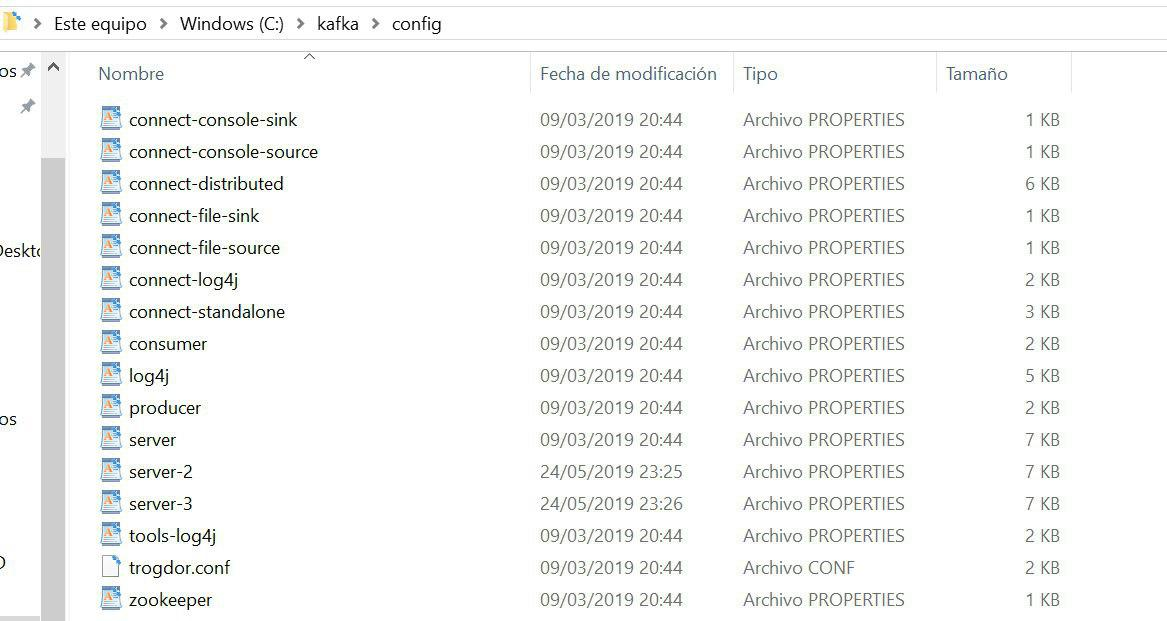
\includegraphics[width=0.8\linewidth]{config_all}
		\caption{Configuración de un cluster de 3 brokers.}
			\end{figure}
\newpage
\subsubsection{Inicio Zookeeper y nodos.}
Mediante consola iniciamos Zookeeper y los brokers.

\begin{figure}[h!]
		\centering
		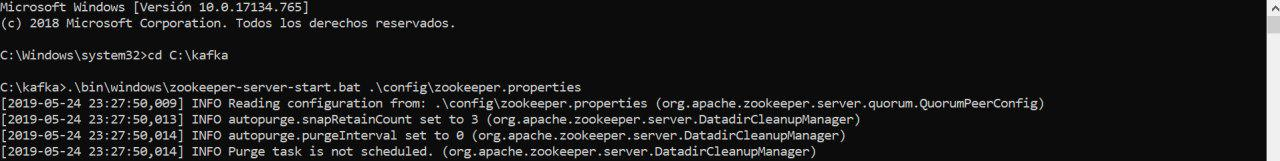
\includegraphics[width=1.1\linewidth]{zookep}
		\caption{Inicio Zookeeper}
			\end{figure}
			
			\begin{figure}[h!]
		\centering
		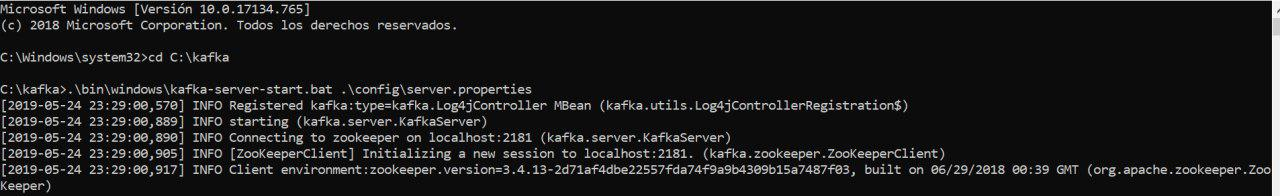
\includegraphics[width=1.1\linewidth]{server}
		\caption{Inicio broker 1}
			\end{figure}
			
			\begin{figure}[h!]
		\centering
		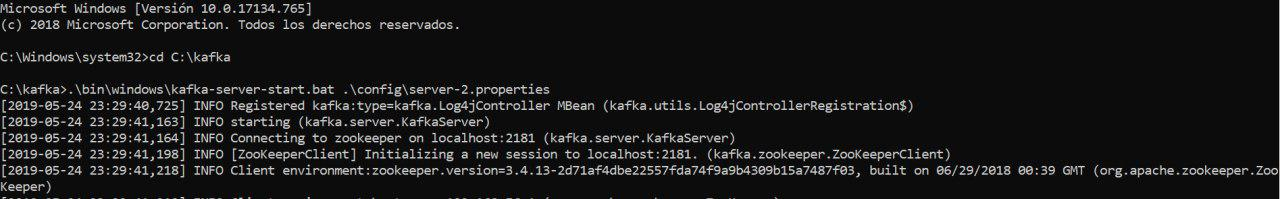
\includegraphics[width=1.1\linewidth]{server2}
		\caption{Inicio broker 2}
			\end{figure}
			\begin{figure}[h!]
		\centering
		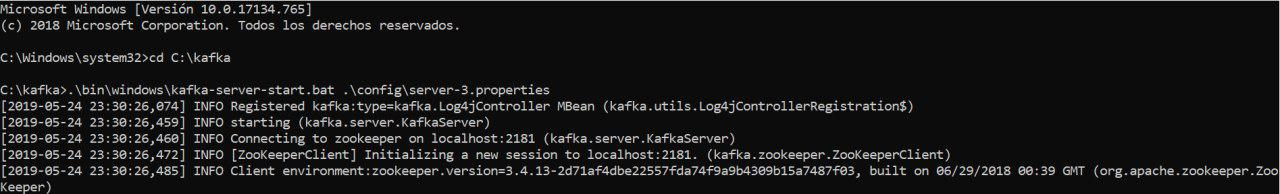
\includegraphics[width=1.1\linewidth]{server3}
		\caption{Inicio broker 3}
			\end{figure}
		
Cabe destacar que no se ha modificado la política de eliminación de mensajes de la configurado por defecto de 168 horas, es decir, una semana.
\newpage
\subsubsection{Scripts}

La arquitectura del sistema consta de un primer productor (Producer\_Tweets.py) que genera el tópic "Tweets" seguido de un consumidor (Consumer\_Producer.py) que se subscribe a éste.  Este consumidor a su vez también actuará como productor generando tres tópics más: \quotes{ClasiNeu},\quotes{ClasiNeg}  y\quotes{ClasiPos} . Por último, tendremos tres consumidores (Consumer\_tweets\_neu.py, Consumer\_tweets\_neg.py y Consumer\_tweets\_pos.py) subscritos, respectivamente, a los tópics anteriores.\\
 De esta forma creamos mediante consola con los scripts de Kafka, los 4 topics que emplearemos a lo largo del trabajo. Se ha decidido crear estos tópics con 2 particiones y factor de replicación 3 para así, trabajar con un sistema resistente a fallos o posibles incidencias.
Ya que el sistema realizará tres copias de los datos de las dos particiones para cada tópic donde cada copia residirá en cada broker. 
De esta forma si el broker con la partición leader del topic se cae, se le podrá asignar otro broker y su partición replica se convertirá en el leader debido al ISR (in-sync replica).\\
Cabe destacar que en la api de confluent kafka para python no se puede determinar el factor de replicación dentro de la configuración del productor, que es el que crea el tópic, por lo que se crean directamente los tópics desde la consola con las características explicadas(fig.6).





\begin{figure}[h]
		\centering
		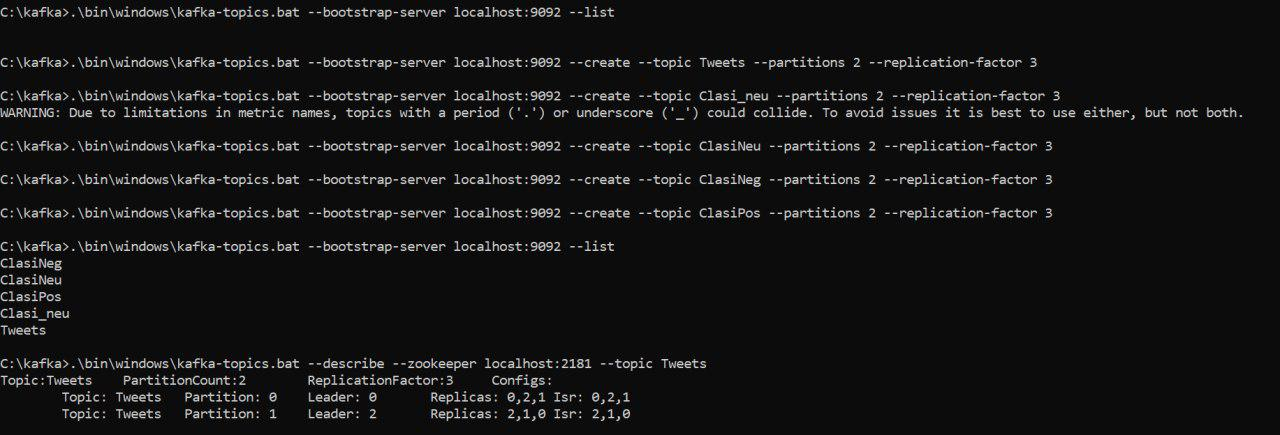
\includegraphics[width=1.1\linewidth]{topic_creation}
		\caption{Creación de los topics}
\end{figure}
Nota: En la imagen hay un error en la creación de los tópics. El tópic \quotes{Clai\_neu} no será utilizado.



Como se deseamos emplear los 3 brokers deberemos tener en cuenta los siguientes parámetros a la hora de configurar los productores, primero creamos la variable\\ KAFKA\_BOOTSTRAP\_SERVERS = "localhost:9092,localhost:9093,localhost:9094", con la configuración de los puertos de cada uno de los brokers y a la hora de crear el productor, le introducimos los siguientes parámetros:
\begin{itemize}
\item 'bootstrap.servers': "KAFKA\_BOOTSTRAP\_SERVERS"
\item $'default.topic.config': {'acks': 'all'}$
\end{itemize}
\newpage
 Empleamos la configuración acks: all , para tener la configuración más fiable ya que de esta forma el broker con la  partición leader espera la confirmación de escritura en todas los brokers de particiones replicas antes de enviar el ACK al productor. Esto garantiza que los mensajes no se pierdan mientras uno de los brokers siga operativo, aunque hace que el procesado sea más lento.\\

Para la configuración de los consumidores también se hará uso de los 3 brokers disponibles, de la misma forma emplearemos como nombre del grupo de consumidores \quotes{Grupo} y haremos uso de las siguientes opciones:
\begin{itemize}
\item 'bootstrap.servers': "KAFKA\_BOOTSTRAP\_SERVERS"
\item 'group.id': \quotes{KAFKA\_CONSUMER\_GROUP}
\end{itemize}


\begin{itemize}
\item \textbf{Producer\_Tweets.py}\\\\ 
En este script se ha emplea la API de Twitter para realizar un stream de los tweets publicados, con filtro que se desee utilizar (modificar el campo $stream.filter(track=['nuevofiltro']))$. De los campos disponibles del tweet publicado nos quedamos con los siguientes: Hora de creación, nombre de usuario, el texto del tweet y el idioma.\\
 Estos campos se guardan en un diccionario y se pasa éste  al consumidor de Kafka asociando los datos al $TOPIC1 = "Tweets"$. Con codificación utf-8. Cada vez que se produzca la captura de un tweet se mostrará en pantalla el siguiente mensaje $'...'$, esto es para corroborar el correcto funcionamiento del script.

		
\item \textbf{Consumer\_producer.py}\\\\
En este script tenemos tenemos un consumidor y un productor, así como una función que viene del paquete de python Vader Sentiment Analysis, que nos permite analizar el contenido de los tweets ya que este paquete esta formado por un lexicon que está especialmente configurado para el analisis de sentimientos con datos de redes sociales y permite procesar los emoticonos.\\
En este script consumiremos el $TOPIC1 = "Tweets"$
y produciremos información en los topics $TOPIC2 = "ClasiNeu"$,$TOPIC3 = "ClasiNeg"$,$TOPIC4 = "ClasiPos"$.\\

De esta forma primero se hace uso de un consumidor que esta suscrito al topic donde se ha codificado la información del productor de  Productor\_tweets y que descodifica los datos en utf-8.\\\\
El siguiente paso realizado es pasar los datos obtenidos del consumidor a la función sentiment\_analyzer\_scores , que evalúa y clasifica el contenido del texto de los tweets mediante el score llamado compount, que contiene la información relativa a la polaridad.\\\\
Finalmente una vez obtenido el score de polaridad haremos uso de un productor que en función del score obtenido tras analizar el sentimiento del Tweet, guardará dicho mensaje en un topic diferente con codificación utf-8.\newpage
 De esta forma:
\begin{itemize}
\item Si la polaridad\textless0, se pasa el mensaje al productor que nos asocia los datos del tweet al $TOPIC3 = "ClasiNeg"$ y mostraremos el mensaje 'Produciendo tweet negativo'
\item Si la polaridad==0, se pasa el mensaje al productor que nos asocia los datos del tweet al $TOPIC2 = "ClasiNeu"$ y mostraremos el mensaje 'Produciendo tweet neutro'
\item Si la polaridad\textgreater0, se pasa el mensaje al productor que nos asocia los datos del tweet al $TOPIC4 = "ClasiPos"$ y mostraremos el mensaje 'Produciendo tweet positivo'
\end{itemize}

La razón detrás de los prints anteriores es para que se pueda observar que está en funcionamiento el script y funciona de forma adecuada.

\item \textbf{Consumer\_tweets\_neu.py}\\\\
Considerando lo realizado anteriormente en el script \textbf{Consumer\_producer.py},
en este script hacemos uso de un consumidor que se suscribe al topic $"ClasiNeu"$ y muestra por pantalla el tweet.
\item \textbf{Consumer\_tweets\_pos.py}\\\\
Considerando lo realizado anteriormente en el script \textbf{Consumer\_producer.py},
en este script, hacemos uso de un consumidor que se suscribe al topic $"ClasiPos"$ y muestra por pantalla el tweet.
\item \textbf{Consumer\_tweets\_neg.py}\\\\
Considerando lo realizado anteriormente en el script \textbf{Consumer\_producer.py},
en este script, hacemos uso de un consumidor que se suscribe al topic $"ClasiNeg"$ y muestra por pantalla el tweet.
\end{itemize}
\newpage
\section{Test de funcionamiento y test de fallo de broker}

Es necesario primero iniciar Zookeeper que es el encargado de la gestión y administración de los distintos brokers, posteriormente se inician los diferentes brokers de Kafka que se vayan a emplear.
Cabe destacar que tanto el inicio de Zookeeper como el de los brokers es necesario realizarlo mediante la consola de windows CMD o Ubuntu Terminal.
El puerto por defecto de Zookeeper es 2181 y para un único broker será el puerto por defecto será 9092.\\

Con Zookeeper en funcionamiento, así como los 3 brokers de Kafka, ahora ponemos en funcionamiento los scripts comentados anteriormente.

El orden adecuado de ejecución es el siguiente:
\begin{itemize}
\item Primero ejecutamos el script \textbf{Producer\_Tweets.py}.
\item Depues ejecutamos el script  \textbf{Consumer\_producer.py}
\item Finalmente ejecutamos los 3 scripts,:\textbf{Consumer\_tweets\_neu.py},\\ \textbf{Consumer\_tweets\_pos.py},\textbf{Consumer\_tweets\_neg.py}
\end{itemize}

En las siguientes imágenes podemos ver la evolución de los topics una vez el código ha estado ejecutándose durante un cierto periodo de tiempo:


\begin{figure}[h]
		\centering
		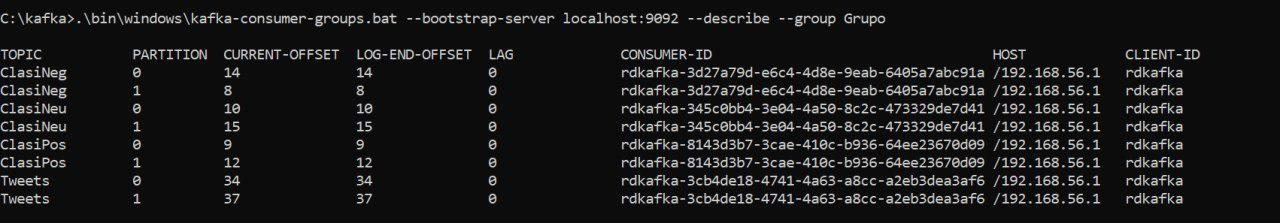
\includegraphics[width=1.1\linewidth]{inicio_codigo}
		\caption{Topics para el broker 1 al inicio}
			\end{figure}
			
			
\begin{figure}[h]
		\centering
		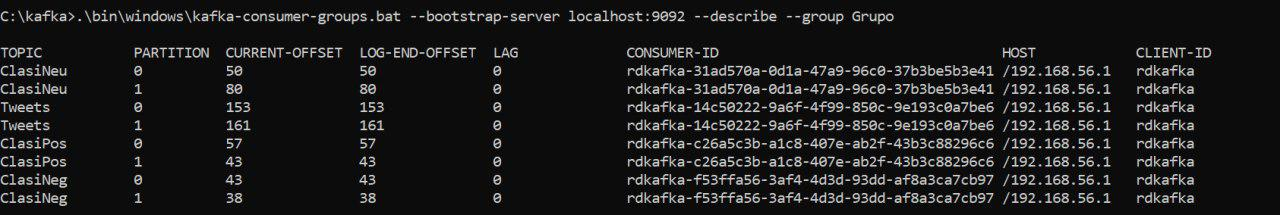
\includegraphics[width=1.1\linewidth]{intermedio_codigo}
		\caption{Evolución del broker 1, tras un periodo de ejecución}
			\end{figure}

\newpage
De la misma forma durante el periodo de captura hacemos un test de fallo de uno de los brokers, concretamente el broker 1(puerto 9092 y broker.id= 0), en el cual se encuentran los topics originalmente y que han sido replicado en los brokers 2 y 3 (puertos 9093 y 9094).


\begin{figure}[h]
		\centering
		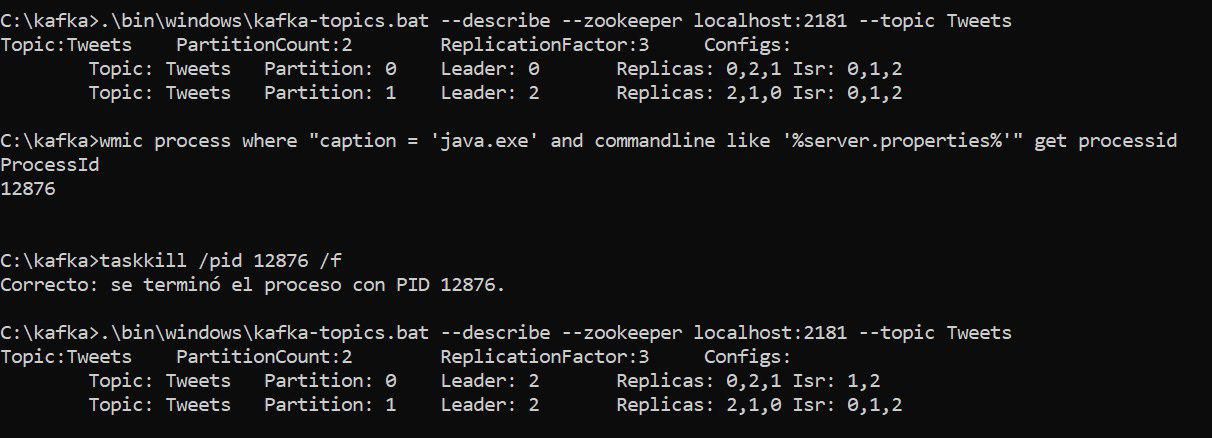
\includegraphics[width=1.1\linewidth]{test_brokerdown}
		\caption{Test de fallo de un broker}
			\end{figure}


Con el comando kafka-topics.bat --describe --zookeeper localhost:2181 --topic tweets , mostramos la información relente sobre el topic que hayamos escogido:
\begin{itemize}
\item Partition: Describe el número de particiones de cada topic.
\item Leader:  Es  el  broker  responsable  de  todas  las  lecturas  y  escrituras  de  cada partición.Indica en que broker se encuentra la replica leader para cada una de las particiones. En nuestro caso, tenemos que para el topic Tweets la replica leader de la partición 0 se encuentra en el broker 2. Ocurre lo mismo para la partición 1.
\item Replicas:  Es  la  lista  de  brokers  que  replican  el  registro  de  esta en cada  partición, independientemente  de  si  son  el  “leader”    o  incluso si  están  actualmente levantados. 
\item Isr: Conjunto de réplicas sincronizadas que están activas y dependen del líder, según la partición. Es decir brokers sincronizados en los que la información está replicada. Como la información esta replicada y sincronizada en los distintos brokers.
\end{itemize}


Se puede observar en la imagen, el topic Tweets inicialmente  para la partición 0 tiene como lider el broker.id=0 y para la partición 1 tiene como lider el broker.id=2. Así como el conjunto de réplicas sincronizadas activas Isr:0,1,2.\\
\newpage
Tras esto ejecutamos el comando wmic process where \quotes{caption = 'java.exe' and commandline like \%server.properties\%'}  get procressid , que nos dice el identificador del proceso del primer broker de Kafka que tenemos corriendo. \\
Y posteriormente ejecutamos el comando taskkill \textbackslash pid "processid" \textbackslash f que nos cierra por consola el broker con broker.id= 0.\\

Tras cerrar el broker 0, para el topic tweets se observa en la imagen como el broker para la replica leader de la partición 0 ha pasado del 0 al 2, es decir, uno de los nodos esclavo anteriores se ha convertido en el nuevo broker "leader". De esta misma forma al matar el broker 0, este ya no se encuentra
en el conjunto de replicas activas , Isr: 1,2.\\



Finalmente tras volver a levantar el broker 0, dejamos corriendo durante más rato todos los scripts. 
Mostramos ahora la descripción final de los topics que contiene cada uno de los brokers:


\begin{figure}[h]
		\centering
		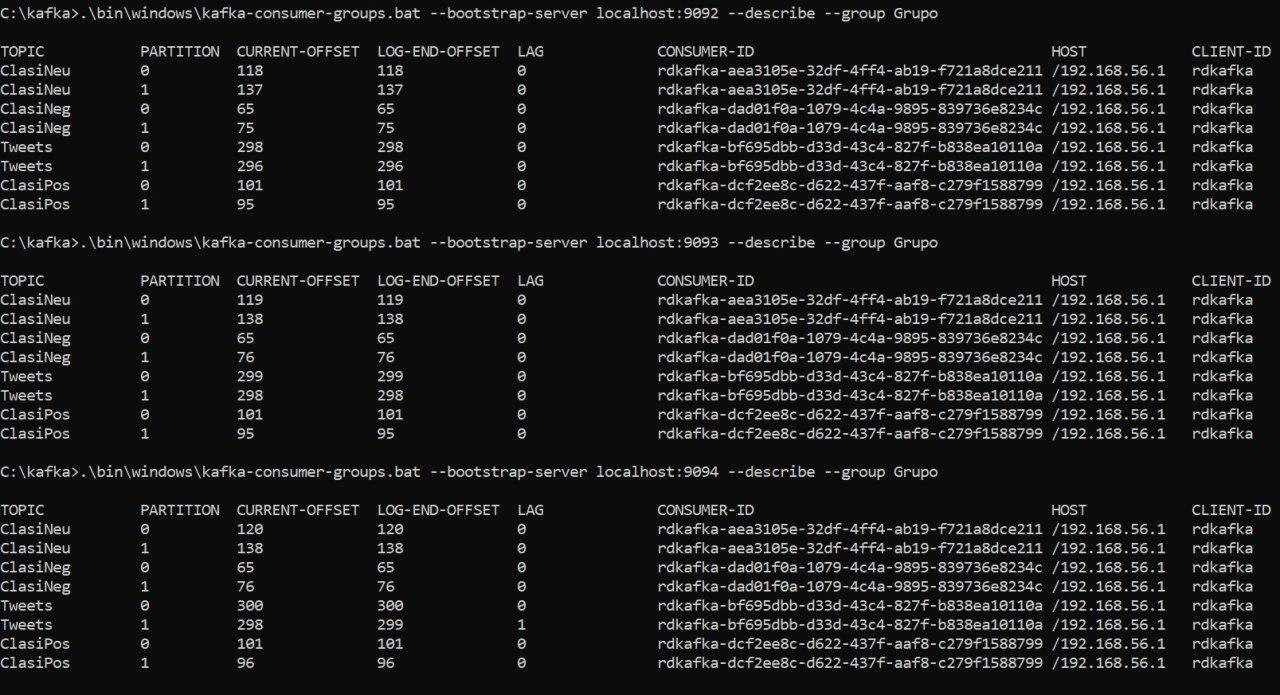
\includegraphics[width=1.1\linewidth]{fin_codigo}
		\caption{Descripción final de los topics por cada broker}
			\end{figure}
\newpage
Si se desease extender este trabajo se podría implementar, en los consumidores que muestran los datos por pantalla de los diferentes tweets en función de su polaridad, un guardado en una base de datos como por ejemplo MongoDB. Donde crearíamos una colección distinta en función de la polaridad. Así aunque cada semana se realizase una limpieza de los topics por la política de eliminación de mensajes configurado en nuestros servidores, mantendríamos los datos a lo largo del tiempo.
Para ello se añadirían las siguientes líneas a los consumidores de los tweets clasificados:\newline


	\begin{verbatim}
	from pymongo import MongoClient
	client = MongoClient('localhost:27017')
	collection = client.mytopic.mytopic
	collection.insert_one(message)
	\end{verbatim}




Donde message sería el mensaje que ha generado el consumer del topic al cual esté suscrito.
\end{document}
